\chapter{Amélioration du workflow de développement}
\epigraph{Il semble que la perfection soit atteinte, non quand il n'y a plus 
rien à ajouter mais quand il n'y a plus rien à retrancher}{--- \small{\textup{Saint-Exupéry,
Terre des hommes}}}

\section{Définition de la mission}
\subsection{Contexte}
Au début de ce stage, mi-juillet, la première tâche fut la prise de contact avec 
les méthodes de travail, les outils utilisés, les logiciels développés, et leurs
\textit{workflows} de développement. En effet, si jusqu'ici seul Studio était développé, Alexis
Pontin venait de terminer le projet du Player, et le développement de Vahana
VR commençait. Studio utilisait alors une architecture de développement particulière
et le Player tout comme Vahana VR commençaient leur développement selon leurs propres
\textit{workflows}.\\
\newline
Ce qui est appelé \textit{workflow} dans ce rapport est un terme pour désigner le 
\enquote{flux de travaux, [c'est-à-dire] une suite de tâches et
d'opérations effectuées par [...] un groupe de personnes}\cite{workflow}, ici l'équipe de développement
de VideoStitch~: c'est une représentation des différentes tâches à accomplir pour, depuis un poste de travail vierge, 
l'installer et pouvoir travailler un des produits de l'entreprise, le compiler et le distribuer.
Ce n'est pas l'architecture des logiciels en eux même, ni leur développement,
mais comment, à partir des sources et des dépendances, il possible d'arriver au produit
compilé et distribuable au client.\\
Ce processus met en \oe uvre les concepts présentés à la section 
\cf{outils-utilisés}. Ils s'articulent ainsi autour du développement
logiciel proprement dit~:\cite{software-build}\cite{build-automation}
\begin{itemize}
  \item La gestion de versions, assurée ici avec Git\cite{gestion-versions}, qui permet
  de récupérer les codes sources.
  \item La chaîne de compilation, dépendante de l'OS cible et automatisée avec Buildbot 
  \cite{chaine-compilation}\cite{integration-continue}.
  \item Les tests d'intégration\cite{integration-continue} réalisés par Buildbot.
  \item La création des installateurs et leur mise à disposition sur une page de téléchargement interne.
\end{itemize}
\ \newline
Cette mission porte essentiellement sur l'amélioration de la chaîne de compilation
pour les applications de VideoStitch, VideoStitch Studio, Vahana VR et VideoStitch
Player, et la création des installateurs. Ce travail a été très complémentaire avec
celui de Jean Duthon, qui a amélioré le \textit{workflow} de développement de VideoStitch SDK,
la gestion des versions et les tests d'intégration.

\subsection{Le \textit{workflow} de développement de VideoStitch Studio}
\label{workflow-studio}
Les codes sources et les dépendances avaient été réparties en quatre dépôts Git~: 
\begin{itemize}
  \item VideoStitch-lib, contenant les codes sources de VideoStitch SDK
  \item VideoStitch-base, contenant des code sources partagés avec le dépôt du VideoStitch Player
  \item VideoStitch-apps, contenant les codes sources de VideoStitch Studio
  \item VideoStitch-deps, contenant les dépendances Windows de VideoStitch Studio 
  nécessaires à sa compilation\footnote{Présentées plus en détails dans \cf{integration-dependances-player}}
\end{itemize}
Sous les systèmes Linux et OS X, il a été décidé d'utiliser les gestionnaires
de paquets apt et Macport pour installer les dépendances logicielles de Studio. Pour
Windows, le dépôt VideoStitch-deps tenait les dépendances sous des versions stables et testées.\\
\newline
Compiler et créer l'installateur de Studio depuis un poste de travail vierge requérait alors
certaines étapes, représentées sous forme d'un diagramme de séquence sur la figure~\ref{workflow-studio}.
Ces étapes étaient essentiellement des appels à des commandes et à des scripts internes
(écrits en bash pour Linux / Mac et en batch pour Windows) pour faire le lien entre les dépôts~:
\begin{enumerate}
  \item Cloner les dépôts VideoStitch-deps, VideoStitch-base et VideoStitch-apps.
  \item Copier, via un script présent sur VideoStitch-base, les codes sources partagés.
  \item Copier, via un script batch présent sur VideoStitch-deps, les dépendances pour Windows.
  \item Récupérer la dernière version du VideoStitch SDK compilée par Buildbot, 
  via un script présent sur VideoStitch-apps.
  \item Générer le Makefile\footnote{Fichier contenant un ensemble de règles destinées
  au compilateur et à l'éditeur de liens.} avec le logiciel qmake, fournis avec Qt.
  \item Compiler avec le logiciel jom\footnote{Ce logiciel fait appel au compilateur 
  du système ainsi qu'à l'éditeur de lien pour générer le logiciel.}, fournis avec Qt.
  \item Générer l'installateur avec un script présent sur VideoStitch-apps.
\end{enumerate}
\begin{figure}
  \centering
  \begin{sequencediagram}
    \footnotesize
    \newthread{u}{Développeur}
    \newinst[1]{a}{VideoStitch-apps}
    \newinst[1]{d}{VideoStitch-deps}
    \newinst[1]{s}{VideoStitch-base}
    \newinst[1]{b}{Buildbot}

    \begin{call}{u}{git clone VideoStitch-apps}{a}{}
    \end{call}
    \begin{call}{u}{git clone VideoStitch-deps}{d}{}
    \end{call}
    \begin{call}{u}{git clone VideoStitch-base}{s}{}
    \end{call}

    \begin{call}{u}{Copy VideoStitch-deps}{d}{}
    \end{call}
    \begin{call}{u}{Copy VideoStitch-base}{b}{}
    \end{call}

    \begin{call}{u}{updatelib.sh}{a}{}
      \begin{call}{a}{Retrieve last SDK}{b}{}
      \end{call}
    \end{call}

    \begin{call}{u}{qmake}{a}{}
    \end{call}
    \begin{call}{u}{make}{a}{return code}
    \end{call}
  \end{sequencediagram}
  \caption{Diagramme de séquence du \textit{workflow} de Studio (juillet 2014)}
	\label{workflow-studio}
\end{figure}
  
\subsection{Problématique}
Représenter ce flux présente l'intérêt de pouvoir ensuite le simplifier et d'automatiser
un maximum des processus requis. Et cela était devenu nécessaire, pour deux raisons~:
\begin{itemize}
  \item L'entreprise commençait sa croissance, impliquant de former les nouveaux arrivants
  à un \textit{workflow} de développement devenue complexe à mesure du temps. Il fallait en
  simplifier le fonctionnement maintenant que Studio et son développement était
  devenus matures\footnote{La première version était sortie, et la bêta de la seconde
  version était en cours}, ce qui permettrait de gagner en efficacité sur le développement
  proprement dit.
  \item Vahana VR et le Player avaient débuté leurs développements; pourtant ces trois
  produits, avec Studio, ont en commun l'utilisation de VideoStitch SDK~: les logiciels
  étant très proches, il était nécessaire d'unifier leurs \textit{worklows} de développement.
\end{itemize}

\subsection{Objectifs}
Les objectifs retenus ont été~:
\begin{itemize}
  \item Faire évoluer le \textit{workflow} de développement vers une gestion multi-logicielle sur le dépôt VideoStitch-apps 
  et en simplifier le fonctionnement.
  \item Intégrer VideoStitch Player et Vahana VR à ce \textit{workflow} de développement.
  \item A cela s'est ajouté, avec le départ d'Alexis, un suivi du Player pour en assurer
  sa maintenance.
\end{itemize}


\section[Réalisation]{Réalisation
\protect\footnote{Nicolas Lopez, Julien Fond et Jean Duthon m'ont beaucoup aidé et, par 
leurs corrections, ont largement contribué aux résultats présentés ici.}}

\subsection{Intégration des dépendances du VideoStitch Player}
\label{integration-dependances-player}
Un programme dépend, pour sa compilation et son exécution, d'autres \emph{paquets} logiciels
\cite{dependance-logicielle}. Ce sont des archives contenant des \emph{bibliothèques logicielles},
c'est-à-dire des ensembles de fonctions déjà compilés et utilisable par le programme.\\
Une bibliothèque logicielle sous Windows se constitue de trois types de fichier\cite{bibliotheque-logicielle}~:
\begin{itemize}
  \item Les \textit{headers} (fichiers .h), qui déclarent les prototypes des fonctions utilisables
  et accessibles de la bibliothèque.
  \item Les bibliothèques (fichiers .lib et .dll), qui contiennent le code des fonctions.
  Les fichiers .lib seront copiés dans le programme, alors que les fichiers .dll seront
  chargés lors du démarrage du programme\cite{bibliotheque-logicielle}.
\end{itemize}
\ \\
En plus d'être spéficique à un système d'exploitation, un programme, et donc
ses dépendances, est spécifique à la plateforme visée (32 bits ou 64 bits)\cite{64-bit-computing}
mais aussi à la configuration compilée (\textit{debug} ou \textit{release})\cite{msdn-debug-release}.\\
La configuration \textit{debug} permet aux développeur de générer une version pour le débogage,
quand la configuration \textit{release} permet de générer une version finale et optimisée destinée
à l'usage du programme. \\
Enfin, le choix de la plateforme dépend du processeur et du
système d'exploitation du client. Les produits de VideoStitch sont distribués
seulement en 64 bits~: les machines pour les faire fonctionner demandent du matériel
récent donc en 64 bits, et cela réduit la maintenante à une seule plateforme.\\
\newline
Le dépôt VideoStitch-deps était déjà logiquement organisé sous la forme présentée par le listing~\ref{videostitch-deps}.
Cette organisation convenait aux nouveaux besoins et a été gardée ainsi. 
\begin{listing}
  \dirtree{%
   .1 /.
   .2 src\DTcomment{Archives des versions des dépendances utilisées}.
   .2 x64\DTcomment{La plateforme 64 bits Windows}.
   .3 bin\DTcomment{Les bibliothèques .dll}.
   .4 debug\DTcomment{Les .dll spécifiques \textit{debug}}.
   .4 release.
   .3 include\DTcomment{Les fichiers \textit{headers} .h}.
   .3 lib\DTcomment{Les bibliothèques .lib}.
   }
  \caption{Dépôt VideoStitch-deps}
  \label{videostitch-deps}
\end{listing}
\ \\
Une séparation
des dépendances par logiciel aurait été possible, mais complexifiant inutilement 
la structure. De plus, les dépendances en commun entre les trois logiciels
sont utilisées dans les même versions. \\
\newline
Ainsi, dans le cadre du Player, deux dépendances ont été ajoutées~:
\begin{itemize}
  \item \textbf{libVLC}~: SDK de VLC, cette bibliothèque fournit des capacités multimédias.\cite{libvlc}
  \item \textbf{Oculus SDK}~: cette bibliothèque permet à une application d'exploiter le 
  casque de réalité virtuelle Oculus Rift.\cite{oculus-developer-guide}
\end{itemize}
Les dépendances Qt et crashrpt\footnote{Envoi de rapports automatiques lors d'un
\textit{crash} du logiciel \url{https://code.google.com/p/crashrpt/}} étaient déjà 
présentes et utilisées par Studio.\\
En parallèle, les dépendances libVLC et Oculus SDK ont été installées sur les Buidlbots Mac et Linux.\\
Quand aux dépendances utilisées par Vahana VR, elles étaient les même que celles 
utilisées Studio, donc déjà présentes dans le dépôt.\\

\subsection{Intégration au \textit{workflow} du VideoStitch Player et de Vahana VR}
La première étape a été de rapatrier le dépôt VideoStitch-base et de l'inclure
avec son historique dans le dépôt VideoStitch-apps. L'annexe \ref{deplacer-historique-depots}
présente plus en détail l'opération permettant, grâce à Git, de déplacer un ensemble 
de fichiers d'un dépôt à un autre tout en préservant l'historique des modifications.\\
De la même manière, furent importés les codes sources de Player et Vahana VR de 
leurs dépôts respectifs.\\
L'opération fut relativement aisée, car le dépôt VideoStitch-apps présentait déjà
une organisation regroupant plusieurs programmes, mais centrés sur le seul logiciel
VideoStitch Studio\footnote{On distingue logiciel et programme, dans le sens où un logiciel
est composé de un ou plusieurs programmes, c'est-à-dire des fichiers binaires, ainsi que des
fichiers de configurations, images, etc.\cite{logiciel}}. L'architecture ne nécessitait alors que quelques modifications, et
a été fixée à la hiérarchie présentée par le listing~\ref{videostitch-apps}.\\
Le dossier de compilation est fixé à \mintinline{shell-session}{bin/x64/<configuration>}
pour tous les systèmes Windows, Linux et Mac OS X.
\begin{listing}
  \dirtree{%
    .1 /.
    .2 bin\DTcomment{Dossier de compilation et dll copiées de VideoStitch-deps}.
    .3 x64.
    .4 debug.
    .4 release.
    .2 installer\DTcomment{Scripts de conception des installateurs}.
    .2 external\_deps\DTcomment{Headers et lib copiés de VideoStitch-deps (Windows)}.
    .3 include.
    .3 lib.
    .2 packager\DTcomment{Scripts de conception des installateurs}.
    .2 src\DTcomment{Codes sources des applications}.
    .3 libvideostitch\DTcomment{Contient les headers copiés du VideoStitch SDK}.
    .3 libvideostitch-base\DTcomment{Programme commun au Player, Studio et Vahana VR}.
    .3 videostitch-player-gui\DTcomment{VideoStitch Player}.
    .3 libvideostitch-gui\DTcomment{Programme commun à Studio et Vahana VR seulement}.
    .3 videostitch-studio-gui\DTcomment{VideoStitch Studio}.
    .3 batchstitcher.\DTcomment{Programme inclus avec Studio}.
    .3 vahana-vr\DTcomment{Vahana VR}.
  }
  \caption{Dépôt VideoStitch-apps}
  \label{videostitch-apps}
\end{listing}
\ \\
L'architecture convenant, les fichiers projets Qt nécessitaient d'être refactorisés,
c'est-à-dire les réécrires pour les adapter aux nouveaux besoins. \\
En effet, les applications Qt définissent des projets (extension .pro) décrivant
les fichiers sources, les ressources et les dépendances utilisées, ainsi que les
paramètres pour le compilateur et l'éditeur de liens (\textit{linker}). Ce sont à 
partir de ces fichiers que le programme qmake construit les instructions de la chaîne
de compilation qui seront éxecutés par jom\cite{qt}. C'est ce qui permet la portabilité
des projets Qt~: un seul projet est écrit, et l'application peut être compilée sur
plusieurs systèmes.\\
Dans ce cas ci, les trois applications étant proches, il était intéressant de partager un maximum de leurs
codes sources sous des programmes communs d'une part et d'autre part de partager
la configuration des différents projets. Les programmes libvideostitch-base et libvideostitch-gui
avaient déjà été définis, regroupant les codes sources communs. 
\ \\
\newline
Enfin, quelques scripts ont été réécrits. Comme vu avec \cf{workflow-studio}, le
développeur doit récuperer la bibliothèque du VideoStitch SDK, et, sur Windows,
les dépendances. Ces ressources se trouvent sur des dépôts séparés, c'est pourquoi
il était nécessaire de pouvoir les récupérer facilement. Git étant l'outil le plus
utilisé pour gérer son code et ses modifications, et son utilisation se réalisant en ligne de commande,
des scripts ont été écrits pour être utilisables comme des commandes en console.\\
De plus tous les scripts batch (pour Windows) ont été supprimés et fusionnés avec
les scripts bash. Si bash est supporté sur tous les Linux et les Mac OS X,
l'utilisation systématique de Cygwin sur Windows par l'équipe a assuré ce support
sur toutes les plateformes.\\
Son utilisation est très simple~: le listing~\ref{update.sh} présente une copie de l'aide affichée.
\begin{listing}
  \begin{minted}[linenos=false]{shell-session}
    Usage: ./updatelib.sh <repository> [configuration]
    Update the actual folder with the required <repository>.

    <repository> is mandatory and other parameters are optionals.
    Parameters can takes the following values:
    <repository>      'deps', 'lib' or 'all' (default)
    [configuration]   'release' (default) or 'debug'
  \end{minted}
  \caption{Aide affichée par la commande ./update.sh}
  \label{update.sh}
\end{listing}
\ \\
Dans le cas de lib, le script va détecter le système de l'utilisateur, puis télécharger avec le programme curl
la dernière version compilée du VideoStitch SDK pour le système et la configuration voulue, pour copier
les headers et les bibliothèques dans les dossiers attendus sur le dépôt VideoStitch-apps.
Le script automatise simplement une action de recherche d'une version compilée par Buildbot
pour en extraire et copier les fichiers.\\
Dans le cas de deps, le script va créer une copie locale de VideoStitch-deps, puis
en copier les headers et les bibliothèques dans les dossiers de VideoStitch-apps.\\
\newline
La figure~\ref{workflow-final} montre la nouvelle utilisation du workflow désormais disponible.
\begin{figure}
  \centering
  \begin{sequencediagram}
    \footnotesize
    \newthread{u}{Développeur}
    \newinst[2]{a}{VideoStitch-apps}
    \newinst[2]{d}{VideoStitch-deps}
    \newinst[2]{b}{Buildbot}

    \begin{call}{u}{git clone VideoStitch-apps}{a}{}
    \end{call}

    \begin{call}{u}{update.sh all}{a}{}
      \begin{call}{a}{git clone VideoStitch-deps}{d}{}
      \end{call}
      \begin{callself}{a}{Copy VideoStitch-deps}{}
      \end{callself}
      \begin{call}{a}{Retrieve last SDK}{b}{}
      \end{call}
    \end{call}

    \begin{call}{u}{qmake}{a}{}
    \end{call}
    \begin{call}{u}{make}{a}{return code}
    \end{call}
  \end{sequencediagram}
  \caption{Diagramme de séquence du \textit{workflow} de développement des applications 
  de VideoStitch (Player, Studio, Vahana VR) (septembre 2014)}
	\label{workflow-final}
\end{figure}

\subsection{Génération des installateurs}
Si la compilation des trois produits est désormais possible, il s'agit désormais
de pouvoir distribuer au client une version finale et utilisable.\\
Le logiciel doit être fournis en version \textit{release} et optimisée, avec ses dépendances associées.
Cependant la compilation produit un certain nombre de fichiers supplémentaires au 
programme compilé, essentiellement pour assister le post-développement du logiciel. 
L'idée est le même sur les trois OS~: il s'agit donc de construire un paquet contenant 
seulement les fichiers nécessaires, le logiciel et ses dépendances.\\
\newline
Le logiciel InnoSetup a été utilisé sur Windows pour générer les installateurs 
des trois applications. Comme pour les projets Qt, les codes des installateurs
on été un maximum mises en commun. Le listing~\ref{inno-setup} présente un exemple
d'une configuration d'installateur, qu'il suffit de passer en argument en ligne
de commande au programme Inno Setup pour générer l'installateur.
\begin{listing}
  \begin{minted}{python}
  [Setup]
  AppName="VideoStitch Player"
  #include "common-setup.iss"

  [Dirs] # will be created and then deleted at uninstall
  Name: "{app}"; Flags: uninuninsalwaysuninstall

  [File] # only necessary files from bin\ will be copied
  Source: "bin\x64\release\videostitch-player.exe"; Destdir: "{app}";
  Source: "bin\x64\release\libvideositch-base.exe"; Destdir: "{app}";
  Source: "bin\x64\release\libvlc.dll"; Destdir: "{app}";
  Source: "bin\x64\release\Qt5*.dll"; Destdir: "{app}";

  [Run]
  Filename: "{app}\vcredistx_64_2013.exe"; Parameters: "/q /norestart"; WorkingDir: "{app}";
  StatusMsg: "Installing Microsoft Visual 2013 (x64) Redistributable Package"
  \end{minted}
  \caption{Extrait de la configuration de l'installateur de VideoStitch Player}
  \label{inno-setup}
\end{listing}
\ \\
De même, les paquet Linux générés sont très simples, comme le présente le listing~\ref{paquet-linux}.
\begin{listing}
  \dirtree{%
    .1 /.
    .2 bin.
    .3 videostitch-player\DTcomment{Le programme}.
    .2 lib.
    .3 libvideostitch-base.so.
    .3 libvlc.so.
    .3 libQt5Core.so.
    .3 libQt5Gui.so.
    .2 launcher\DTcomment{Lance le programme après initialisation des librairies}.
  }
  \caption{Paquet Linux de VideoStitch Player}
  \label{paquet-linux}
\end{listing}

\subsection{Automatisation de la chaîne de compilation}
La génération des installateurs Windows et des paquets Linux / Mac est cependant
toujours fastidieuse et gagnerait à être automatisée. L'équipe se concentre avant
tout au développement, quand l'intégration continue est réalisée par Buildbot. 
Il s'agit désormais d'écrire les routines pour permettre à Buildbot de générer
les quatre produits de VideoStitch ainsi que leurs installateurs.\\
Deux concepts sont importants dans Buildbot~: les \textit{builders} et les \textit{schedulers}.
Les premiers sont la suite des étapes à accomplir pour générer les logiciels, quand
les seconds sont ceux qui vont lancer ces \textit{builders}. Après une modification
sur un dépôt, ou après la fin d'un \textit{builder}~: par exemple, après la compilation de
VideoStitch SDK, les applications sont générées pour tester le bon fonctionnement
du SDK.\\
Le système de \textit{schedulers} et de \textit{builders} étant déjà créé pour 
générer Studio sur Windows, Mac et Linux, il suffisait de rajouter les différentes 
étapes pour générer le Player et Vahana VR. Ces étapes sont écrites en Python dans un fichier de configuration.
L'usage est intéressant~: chaque modification de la configuration recquiert ensuite d'utiliser la commande
\mintinline{shell-session}{buildbot reconfig} qui va prévenir si la configuration
contient des erreurs ou non.\\
\newline
Pour exemple, le listing~\ref{windows-apps} présente un extrait de l'utilisation 
du \textit{builder} du dépôt VideoStitch-apps pour Windows, qui a été précédemment 
définis avec l'id \mintinline{shell-session}{windows_apps}~:
\begin{listing}
  \begin{minted}{python}
  windows_apps = BuildFactory() # Initiate a new build
  windows_apps.addStep(getGitRepo("apps", "git@github-apps.com:VideoStitch/VideoStitch-apps.git"), descriptionDone=["Update from the Git repository VideoStitch-apps"])
  windows_apps.addStep(ShellCommand(command=["bash", "update.sh", "all", "release"], descriptionDone=["Update lib and deps"], workdir="VideoStitch-apps"))
  windows_apps.addStep(ShellCommand(command=["qmake", "CONFIG+=release"], workdir="VideoStitch-apps/src/vahana-vr", descriptionDone=["Generate Makefile for Vahana"])
  windows_apps.addStep(ShellCommand(command=["make"], workdir="VideoStitch-apps/src/vahana-vr", descriptionDone=["Building Vahana VR"]))
  \end{minted}
  \caption{Extrait du \textit{builder} Windows sur le Buildbot}
  \label{windows-apps}
\end{listing}

\subsection{Maintenance du VideoStitch Player}
Enfin, quelques apports mineurs et rapides ont été apportés, pour améliorer l'usage
du Player lors des présentations dans les salons et conférences.
\subsubsection{Support de l'Oculus Rift DK2}
Le player propose deux modes de vues, comme présenté dans la section \cf{videostitch-player-section}~:
une vue interactive, avec un déplacement dans la sphère 360 avec la souris et un affichage
sur un écran standard, et une seconde vue utilisant le casque de réalité virtuelle 
Oculus Rift pour le déplacement et l'affichage, créant une vue totalement immersive.\\
En juillet 2014\cite{dk2s-now-shipping}, est sortie la nouvelle version dite DK2 de ce casque encore
en développement. Le Player se devait de supporter cette nouvelle version.\\
Dans un premier temps, après réception du casque, les drivers Oculus ont été mis à
jour et le bon fonctionnement du casque a été testé. Une nouvelle version de l'Oculus
SDK avait été mise à disposition, VideoStitch-deps a donc été mis à jour avec les nouvelles
bibliothèques et \textit{headers} tout comme les machines Buildbot Mac et Linux.\\
\newline
Une classe \mintinline{c++}{OculusRift} avait déjà été définie pour permettre l'utilisation
de l'Oculus SDK. Après la lecture de la documentation de ce SDK et celle du code,
le Player a été mis à jour pour utiliser l'API de cette nouvelle version, assurant
ainsi le support du DK1 et du DK2.

\subsubsection{Passer le \textit{Health and Safety Warning} de l'Oculus}
Le nouvel Oculus SDK a vu l'apparition de nouvelles clauses légales et d'un écran
d'avertissement appellé \textit{Health and Safety Warning}, tel que sur la figure~\ref{hsw-oculus}
lors du démarrage d'une vidéo dans le casque\cite{oculus-developer-guide}.\\
Il s'agissait alors d'ajouter une possibilité de passer cet écran, en pressant une
manuellement une touche du clavier. Cela ne pouvait être fait automatiquement afin de respecter les clauses.
\begin{figure}
  \centering
  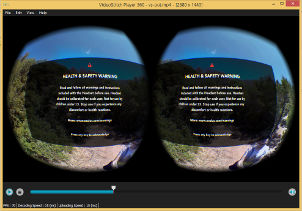
\includegraphics[width=8cm]{images/player-oculus-hsw.jpg}
  \caption{L'écran \textit{Health and Safety Warning} affiché par l'Oculus Rift}
  \label{hsw-oculus}
\end{figure}
\ \\
L'implémentation se réalisa avec la création d'une fonction pour désactiver le HSW
(listing~\ref{player-oculusrift}) et avec une capture d'une touche du clavier pour faire appel à 
cette fonction (listing~\ref{player-mainwindow}) via le système signal/slot de Qt.\\
La classe \mintinline{c++}{OculusRift} propose une gestion de l'oculus et une utilisation
à l'ensemble de l'application du Player, via un certain nombre de fonctions publiques
et de slots Qt\footnote{Un slot est une fonction pouvant être appellée de manière asynchrone 
par un signal provenant de la même classe ou d'une autre.}. La fenêtre principale \mintinline{c++}{MainWindow}
de l'application utilise la fonction prédéfinie \mintinline{c++}{keyPressEvent} fournie
par Qt qui \enquote{écoute} les touches pressées par l'utilisateur dans le Player.
Ici, quelque soit la touche, un signal est envoyé pour demander la désactivation du HSW.
\begin{listing}
  \begin{minted}[firstnumber=109]{c++}
    void OculusRift::disableHSW() {
      ovrHSWDisplayState hsw;
      ovrHmd_GetHSWDisplayState(hmd, &hsw);
      if (hsw) {
        ovrhmd_EnableHSWDisplaySDKRender(hmd, false); // hmd object manages the oculus
      }
    }
  \end{minted}
  \caption{Extrait du fichier oculusrift.cpp}
  \label{player-oculusrift}
\end{listing}

\begin{listing}
  \begin{minted}[firstnumber=90]{c++}
  connect(this, SIGNAL(disableOculusHSW()), oculusRift, SLOT(disableHSW()));
  
  void MainWindow::keyPressEvent(QKeyEvent *e) { // 
    emit disableOculusHSW();
  }
  \end{minted}
  \caption{Extrait du fichier mainwindow.cpp}
  \label{player-mainwindow}
\end{listing}


\section{Bilan et suite}
Cette première mission occupa les premiers mois du stage, et permis d'acquérir
le fonctionnement du \textit{workflow} de développement de l'entreprise afin de l'améliorer.
Les modifications apportées, même si elles ont été parfois mineures, ont cependant permis dans leur globalité~:
\begin{itemize}
 \item De compiler depuis un même dépôt, quelque que soit l'OS de la machine, les trois applications de VideoStitch.
 \item D'automatiser la compilations et la génération des paquets de ces trois applications 
 sur Buidlbot, rendant les dernières versions immédiatement utilisables par n'importe 
 quelle personne de VideoStitch.
 \item D'apporter les modifications nécessaires à l'usage du Player.
 \item De permettre une installation d'un nouvel environnement de développement et
 de sont usage relativement aisé, comme le montre la figure~\ref{workflow-final}.
\end{itemize}
\ \\
Ce système pourrait encore être amélioré, ou même à être repris de zéro. Cependant, 
une telle réécriture demanderait nécessairement beaucoup plus de temps pour
produire un système certes plus correct au regard des besoins actuels, mais moins mature
et donc plus sujet à des cas d'utilisations non prévus ou problématiques. De plus,
il aurait fallu changer les habitudes de l'équipe de développement.\\
Cependant, des cas d'utilisations non prévus sont également apparus lors de cette mission,
mais sont rapidement corrigés par l'équipe. Bien souvent, cela est dû à des différences
d'interprétations du bash entre Linux et Mac OS X, ou par une différence de code avec
le script batch correspondant. Les scripts pourraient alors être écrits en Python, pour
éviter ces différences et ces erreurs. Leur écriture et leur maintenance serait 
en outre facile, Python étant relativement simple dans son approche et ses usages.\\
Enfin, VideoStitch Player nécessiterait d'être amélioré~: la vidéo
4K n'est pas encore correctement lue, et le logiciel gagnerait à être finis lors
de quelques sprints de l'équipe.
